% ====chapter=====
\myChapter{Mise en oeuvre et évaluation de ProOWeb}{}
\label{chap:mise-oeuvre-evaluation-prooweb}
\myMiniToc{mysection}{Sommaire}

\mySection{Introduction}{}

Le chapitre précédent a présenté le framework proposé pour générer une application web métier à partir d'un modèle BPMN complété par une spécification applicative. Il a notamment défini l'architecture générale de ProOWeb, le rôle de \textit{spec-v1}, les transformations modèle-à-modèle et modèle-à-texte, ainsi que les mécanismes de préservation du code personnalisé. Nous passons maintenant de cette description d'ensemble à sa mise en oeuvre, en observant comment ProOWeb produit une application métier destinée à une organisation de commerce électronique.

Le chapitre suit donc le chemin emprunté par le framework : initialisation du projet, modélisation ou importation des processus, validation des spécifications enrichies, déploiement des contrats runtime et data, génération des artefacts backend/frontend et vérification des parcours obtenus. Cette progression permet de relier le modèle conceptuel du chapitre \ref{chap:framework-prooweb} au résultat produit dans l'application générée.

\mySection{Environnement de mise en oeuvre}{}
\label{sec:chap4-environnement}

\subsection{Objectif de réalisation}

La mise en oeuvre de ProOWeb a consisté à rendre opérationnel le framework décrit au chapitre précédent. Les blocs conceptuels présentés dans l'architecture de la section \ref{sec:chap3-architecture} sont ici traduits en composants réalisés : un noyau de génération, des mécanismes de validation, des contrats intermédiaires, des gabarits et un projet applicatif cible. Le framework reçoit des informations métier structurées, vérifie leur cohérence, construit des contrats intermédiaires et produit une base applicative exploitable. Cette base contient les éléments nécessaires pour exécuter un processus, afficher les tâches, appliquer les rôles, manipuler les données et suivre les fichiers générés.

Dans ce travail, ProOWeb n'est donc pas présenté comme une simple maquette. Il sert à vérifier si le passage du modèle BPMN vers une application web métier peut être automatisé tout en gardant une trace claire entre le besoin métier et les artefacts produits.

\subsection{Choix technologiques}

Le générateur a été séparé de l'application produite. Cette séparation reprend la distinction établie au chapitre \ref{chap:framework-prooweb} entre le noyau de génération et l'application web générée. ProOWeb s'exécute comme une application Node.js. Il fournit une interface de configuration, des services de gestion du workspace et des modules spécialisés dans la modélisation de processus : catalogue, validation de \textit{spec-v1}, simulation, déploiement, génération des contrats runtime et gestion des fichiers produits.

L'application générée, quant à elle, repose sur Spring Boot pour le backend, React/Vite pour l'interface web et PostgreSQL comme base de données cible. Le workspace généré pour le cas d'étude porte le nom E-commerce Application. Il active notamment la modélisation de processus, la hiérarchie organisationnelle, les notifications, Liquibase, Swagger en profil de développement, les scripts de lancement et les tests frontend Cypress. Ce choix technique n'est donc pas seulement déclaratif : il correspond à une arborescence générée, à des fichiers de configuration et à des scripts de vérification présents dans le projet.

\begin{table}[H]
\centering
\caption{Principaux choix de mise en oeuvre de ProOWeb}
\label{tab:chap4-choix-techniques}
\begin{tabularx}{\textwidth}{p{3.0cm}p{3.3cm}X}
\toprule
\textbf{Éléments} & \textbf{Choix retenu} & \textbf{Rôle dans ProOWeb} \\
\midrule
Noyau du framework & Node.js / JavaScript & Lire le workspace, importer les modèles, valider \textit{spec-v1}, construire les contrats et déclencher le déploiement. \\
Interface de configuration & Pages web ProOWeb & Initialiser le projet, accéder au tableau de bord et piloter certaines opérations de génération. \\
Backend généré & Spring Boot modulaire & Porter les modules système, organisation, sécurité, runtime de processus et ressources métier générées. \\
Frontend généré & React/Vite & Fournir les vues de travail, notamment le \textit{Process Runtime Workbench} utilisé dans les tests. \\
Base de données cible & PostgreSQL avec Liquibase & Préparer la persistance et les scripts de migration nécessaires au projet produit. \\
Suivi des fichiers & Manifeste de génération & Identifier les fichiers générés et soutenir les régénérations contrôlées. \\
Vérification & Scripts et tests Cypress & Vérifier les parcours frontend liés aux processus déployés. \\
\bottomrule
\end{tabularx}
\end{table}

\subsection{Organisation réalisée}

ProOWeb est organisé autour de deux espaces qui gardent chacun une responsabilité claire. D'un côté, le framework contient les services de lecture des modèles, les validations, la construction des contrats, les gabarits et les mécanismes de suivi. De l'autre, le projet cible regroupe les fichiers applicatifs produits à partir des modèles et destinés à être exécutés, testés puis adaptés.

Cette séparation se voit directement dans l'arborescence du projet. Les modules du framework sont placés dans \texttt{ProOWeb/src/lib} et \texttt{ProOWeb/src/services}. Les artefacts générés sont présents dans le workspace applicatif, avec un backend Spring Boot, un frontend React et des ressources de processus rangées dans le dossier \texttt{resources/processes} du module applicatif. Pour chaque processus déployé, ProOWeb conserve le BPMN, une spécification transformée, un contrat runtime et un contrat de données. Cette organisation rend le résultat plus lisible : le modèle d'entrée reste consultable, tandis que les contrats générés expliquent comment le modèle est projeté vers l'application.

\begin{table}[H]
\centering
\caption{Organisation fonctionnelle réalisée dans ProOWeb}
\label{tab:chap4-organisation-realisee}
\begin{tabularx}{\textwidth}{p{3.6cm}X}
\toprule
\textbf{Bloc} & \textbf{Responsabilité principale} \\
\midrule
Workspace généré & Conserver la configuration de l'application e-commerce, les scripts et les modules générés. \\
Catalogue de processus & Enregistrer les modèles, les versions, les statuts de validation et les informations de déploiement. \\
Validation \textit{spec-v1} & Refuser ou signaler les incohérences entre le BPMN, les rôles, les données et les activités enrichies. \\
Contrats runtime et data & Préparer une représentation stable des activités, transitions, rôles, données partagées et règles d'accès. \\
Ressources backend & Déposer les fichiers \texttt{v1.bpmn}, \texttt{v1.json}, \texttt{v1.runtime.json} et \texttt{v1.data.json} par processus. \\
Manifeste & Garder la mémoire des fichiers générés afin de contrôler les évolutions ultérieures. \\
\bottomrule
\end{tabularx}
\end{table}

\mySection{Implémentation de la chaîne de génération}{}
\label{sec:chap4-implementation-generation}

La figure \ref{fig:chap4-chaine-generation} présente la chaîne de génération
mise en oeuvre dans ProOWeb. Elle reprend les étapes conceptuelles décrites dans
la section \ref{sec:chap3-transformations} : lecture des modèles, validation,
construction d'une représentation intermédiaire, projection vers les artefacts et
suivi de la génération. Elle montre ainsi le passage des modèles d'entrée vers
les contrats intermédiaires, puis vers les artefacts applicatifs et le manifeste
de traçabilité utilisé lors des régénérations.

\begin{figure}[H]
\centering
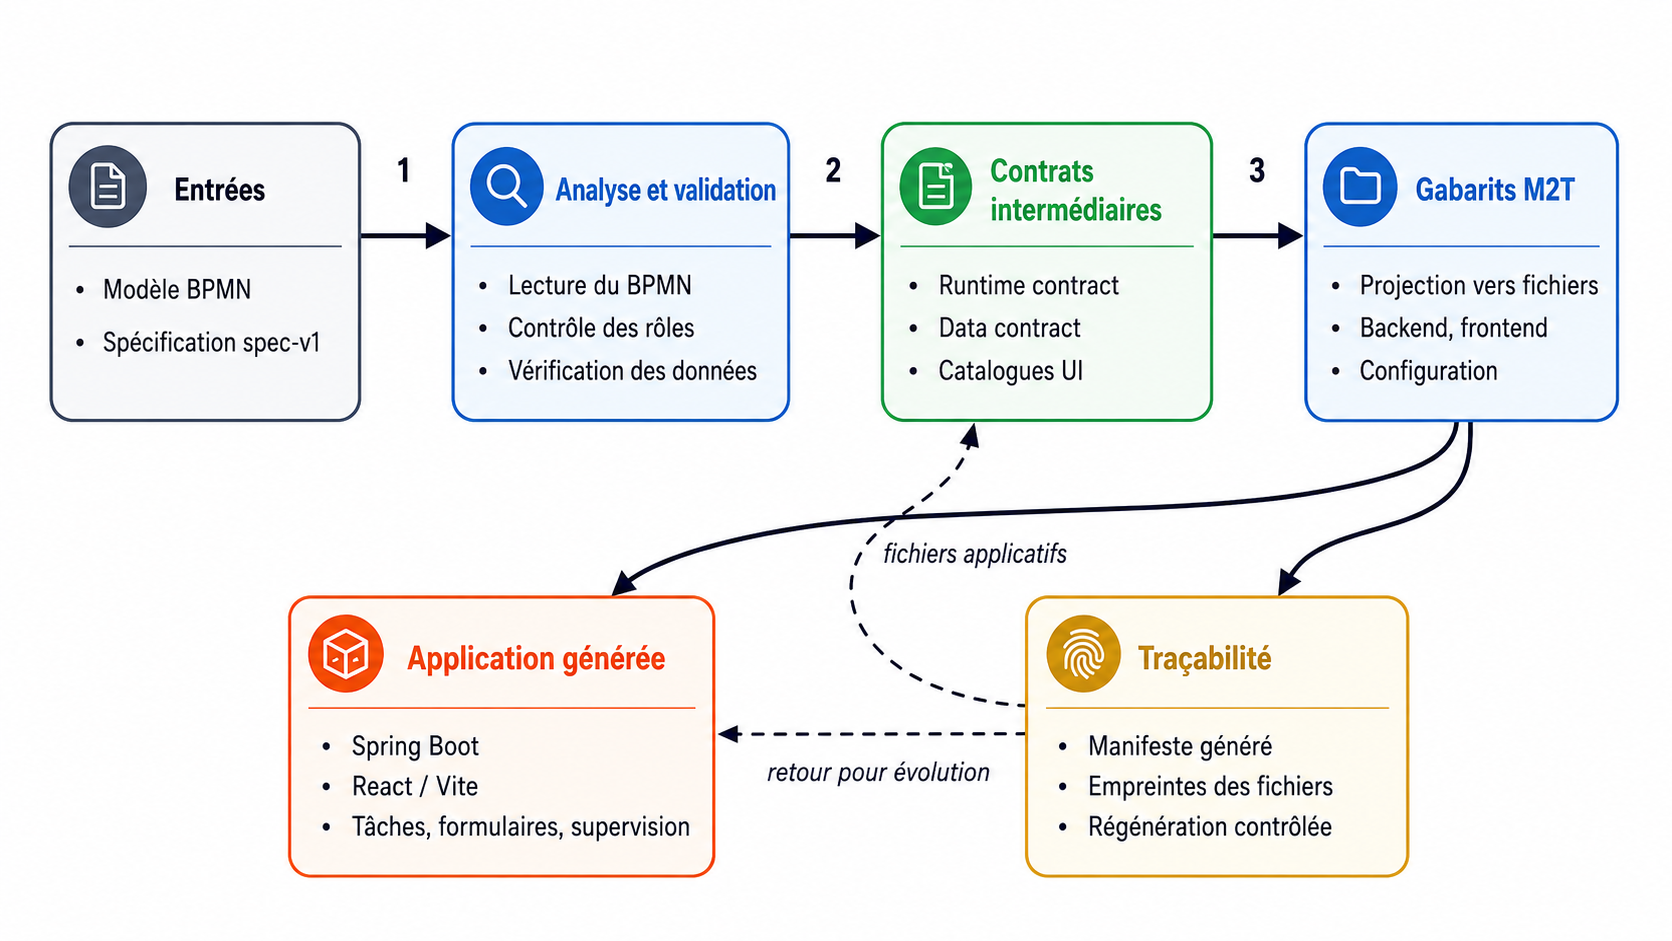
\includegraphics[width=0.75\textwidth]{Chap4/images/image2.png}
\caption{Chaîne de génération de ProOWeb}
\label{fig:chap4-chaine-generation}
\end{figure}


\subsection{Initialisation du projet cible}

La génération commence par l'initialisation du projet cible. Cette étape fixe l'identité de l'application à produire : nom du projet, espace de travail, package de base, options d'authentification, profils d'exécution et paramètres généraux. Dans le cas d'étude, cette initialisation a produit le workspace E-commerce Application, avec le package de base \texttt{com.prooweb.generated}, un backend Spring Boot, un frontend React et une base de données cible PostgreSQL.

\begin{figure}[H]
\centering
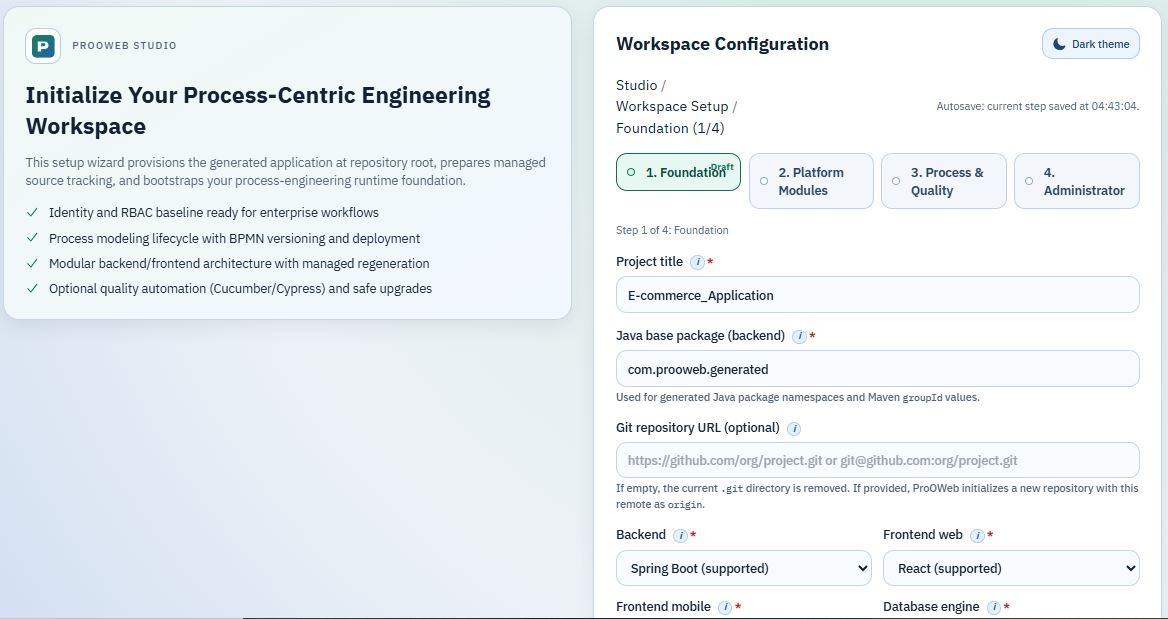
\includegraphics[width=0.75\textwidth]{Chap4/images/image1.JPG}
\caption{Initialisation du projet \texttt{E-commerce\_Application}}
\label{fig:chap4-initialisation-projet}
\end{figure}

Cette étape prépare une application structurée, équipée de scripts de compilation, de vérification, de test et de lancement par profil. Le workspace contient ainsi les scripts \texttt{build-all}, \texttt{test-all}, \texttt{verify-all} et \texttt{start-profile}, ainsi que les raccourcis NPM qui permettent de piloter ces opérations depuis la racine du projet.

\subsection{Gestion des modèles de processus}

Après l'initialisation, ProOWeb prend en charge les modèles BPMN et les spécifications \textit{spec-v1}. Le BPMN garde le rôle de support de workflow. La spécification enrichie ajoute les informations que le modèle ne porte pas naturellement : rôles candidats, règles d'affectation, entrées, sorties, données partagées, visibilité et stratégies de stockage.

Pour le cas d'étude, les trois BPMN et les trois fichiers de spécification conservés dans le chapitre 4 sont importés dans ProOWeb par un script dédié. Ce script lit les sources, normalise certaines informations, transforme la spécification de travail vers la forme attendue par ProOWeb, puis lance la validation stricte avec le catalogue des tâches automatiques. Lorsque le modèle est recevable, une version est créée ou ajoutée dans le catalogue, simulée, puis déployée. Cette étape donne une valeur particulière au cas d'étude : les processus présentés dans le mémoire ne restent pas au niveau du dessin, ils deviennent des versions de processus manipulées par le framework.

\subsection{Validation et construction des contrats}

La validation est le premier point de contrôle sérieux de la chaîne. Elle met en oeuvre les contrôles introduits dans le chapitre précédent : cohérence entre BPMN et \textit{spec-v1}, présence des rôles nécessaires, validité des données et correspondance entre activités et artefacts à produire.

Lorsque ces contrôles sont satisfaits, ProOWeb construit des contrats intermédiaires. Ces contrats correspondent à la matérialisation du modèle pivot présenté au chapitre \ref{chap:framework-prooweb}. Dans le workspace généré, ils apparaissent sous la forme d'un catalogue runtime, d'un catalogue de données, d'un catalogue de tâches automatiques et de contrats propres à chaque processus. Ils ne sont pas encore le comportement exécuté par un utilisateur, mais ils donnent au générateur une base stable pour produire les vues, les règles de progression et les données partagées.

\begin{table}[H]
\centering
\caption{Contrats produits avant la génération des fichiers}
\label{tab:chap4-contrats-generation}
\begin{tabularx}{\textwidth}{p{3.7cm}X}
\toprule
\textbf{Contrat} & \textbf{Utilisation dans ProOWeb} \\
\midrule
\textit{Runtime contract} & Décrire les processus, activités, transitions, statuts et actions disponibles pendant l'exécution. \\
\textit{Data contract} & Organiser les données partagées, les champs, les sources et les mappings issus des activités. \\
Catalogue des formulaires & Définir les champs affichés, les champs produits et les contraintes des activités manuelles. \\
Catalogue d'interface & Préparer les vues utiles : listes de tâches, actions, suivi et règles d'affichage. \\
Registre des processus & Conserver les processus disponibles, leurs versions et leurs métadonnées d'exploitation. \\
\bottomrule
\end{tabularx}
\end{table}

\subsection{Génération des artefacts applicatifs}

La génération transforme les contrats en fichiers organisés dans le projet cible. Elle concrétise les règles de projection décrites au chapitre précédent : une activité, un rôle, une transition ou une donnée partagée sont traduits en artefacts applicatifs cohérents. Une activité BPMN enrichie ne devient donc pas seulement une ligne dans un fichier de configuration. Elle donne lieu à un ensemble cohérent : une action de traitement, un formulaire, des contrôles d'accès, des transitions de processus et des traces exploitables dans l'historique.

Le résultat attendu est une base applicative cohérente, et non une collection de fichiers isolés. Les artefacts produits sont regroupés autour de besoins simples : exécuter un processus, faire traiter les tâches, conserver les informations, contrôler les accès et suivre l'évolution du projet généré.

\begin{lstlisting}[breaklines=true,caption={Organisation simplifiée du workspace généré},label={lst:chap4-arborescence-generee}]
E-commerce_Application/
  src/
    backend/
      springboot/
        common/
        organization/
        system/
        prooweb-application/
          src/main/resources/processes/
    frontend/
      web/react/
        src/
        cypress/e2e/
  deployment/
    docker/
  build-all.ps1
  test-all.ps1
  verify-all.ps1
  start-profile.ps1
  .prooweb-managed.json
\end{lstlisting}

\subsection{Préservation et régénération contrôlée}

ProOWeb met en place un manifeste des fichiers générés. Ce choix prolonge les mécanismes de préservation et de synchronisation discutés dans la section \ref{sec:chap3-preservation}. Le manifeste garde la trace des chemins, des catégories et des empreintes associées aux fichiers produits. Lorsqu'une nouvelle génération est lancée, le framework peut comparer l'état attendu avec l'état présent dans le projet cible.

Ce mécanisme répond à une difficulté réelle : une application générée n'est pas figée. Une équipe peut modifier un libellé, ajouter une règle locale, connecter un service externe ou adapter une vue. La régénération ne doit donc pas effacer ces interventions sans contrôle. ProOWeb cherche à garder le lien entre modèle et code tout en respectant les adaptations humaines.

\begin{lstlisting}[breaklines=true,caption={Extrait simplifié du manifeste de génération},label={lst:chap4-manifeste}]
{
  "generatedAt": "2026-06-25",
  "files": [
    {
      "path": "src/backend/.../processes/commande-client/v1.runtime.json",
      "source": "commande-client:v1",
      "category": "process-runtime-contract",
      "managed": true
    },
    {
      "path": "src/frontend/web/react/cypress/e2e/process-commande-client-v1.cy.js",
      "source": "commande-client:v1",
      "category": "frontend-e2e-test",
      "managed": true
    }
  ]
}
\end{lstlisting}

\mySection{Cas d'étude organisationnel}{}
\label{sec:chap4-cas-etude}

\subsection{Présentation de l'organisation retenue}

Le cas d'étude retenu concerne une organisation de commerce électronique. Cette organisation vend des produits à travers une boutique en ligne et s'appuie sur plusieurs pôles internes : prise en charge des commandes, gestion du stock, préparation logistique, service client et supervision commerciale. Son activité ne se résume donc pas à l'affichage d'un catalogue. Elle implique des décisions, des contrôles, des validations et des échanges entre acteurs avant qu'une commande soit clôturée ou qu'une réclamation soit traitée.

Ce terrain est intéressant pour ProOWeb parce que les processus ne sont pas isolés. Une commande client peut consommer du stock ; une rupture peut déclencher un réapprovisionnement ; une réclamation peut concerner une commande déjà livrée et nécessiter une vérification commerciale ou logistique. Le cas d'étude permet ainsi de vérifier si une même application générée peut regrouper plusieurs workflows tout en conservant une cohérence métier autour des clients, des produits, des commandes et des mouvements de stock.

Ce cas d'étude sert donc de terrain d'application aux choix de conception présentés dans le chapitre \ref{chap:framework-prooweb}. Les processus retenus permettent d'observer l'utilisation conjointe du BPMN, de la spécification \textit{spec-v1}, des contrats intermédiaires, des règles de projection et du mécanisme de traçabilité.

\subsection{Acteurs et responsabilités}

Les acteurs retenus correspondent aux responsabilités courantes d'une organisation de commerce électronique.
\begin{table}[H]
\centering
\caption{Acteurs du cas d'étude e-commerce}
\label{tab:chap4-acteurs-cas-etude}
\begin{tabularx}{\textwidth}{p{2.8cm}p{4.2cm}X}
\toprule
\textbf{Acteur} & \textbf{Responsabilité principale} & \textbf{Interaction avec l'application générée} \\
\midrule
Client & Passer une commande ou déposer une réclamation de produit & Renseigne les informations nécessaires et suit l'état de ses demandes. \\
Service commercial & Suivre les commandes et arbitrer les cas nécessitant une décision & Consulte les commandes, confirme certaines décisions et suit les exceptions. \\
Gestionnaire de stock & Vérifier les disponibilités, préparer les commandes et enregistrer les mouvements & Reçoit les tâches liées au stock, à la préparation et à la réception des produits. \\
Responsable achats & Valider les réapprovisionnements et suivre les demandes fournisseur & Examine les besoins de stock et autorise les commandes d'achat. \\
Service client & Qualifier les réclamations de produit et proposer une solution & Traite les demandes après-vente et renseigne les décisions prises. \\
Administrateur & Configurer les rôles, produits, catégories et paramètres généraux & Maintient les données de base utilisées par les processus générés. \\
\bottomrule
\end{tabularx}
\end{table}

\subsection{Processus retenus}

Trois processus ont été retenus pour représenter le fonctionnement de cette organisation. La commande client couvre le parcours qui va de la soumission de la commande à sa préparation. Le réapprovisionnement du stock intervient lorsqu'un produit devient insuffisant ou lorsqu'un responsable anticipe une rupture. La réclamation de produit prend en charge les demandes formulées après une vente. Ces processus partagent des données et des acteurs, mais ils répondent à des objectifs opérationnels différents.

\begin{table}[H]
\centering
\caption{Processus métier retenus dans le cas d'étude}
\label{tab:chap4-processus-retenus}
\begin{tabularx}{\textwidth}{p{2.5cm}p{3.6cm}p{2.7cm}X}
\toprule
\textbf{Processus} & \textbf{Objectif métier} & \textbf{Acteurs clés} & \textbf{Résultat observé} \\
\midrule
P1 : commande client & Recevoir, vérifier, préparer et clôturer une commande passée sur la boutique en ligne & Client, service commercial, gestionnaire de stock & Commande confirmée, préparée, annulée ou clôturée. \\
P2 : réapprovisionnement du stock & Détecter un besoin de stock, le faire valider et enregistrer la réception des produits & Gestionnaire de stock, responsable achats & Stock réapprovisionné ou demande refusée. \\
P3 : réclamation de produit & Traiter une réclamation liée à une commande et proposer une solution adaptée & Client, service client, service commercial, gestionnaire de stock & Réclamation clôturée avec décision tracée. \\
\bottomrule
\end{tabularx}
\end{table}

\subsection{Déroulement des scénarios}

Le processus P1 commence lorsqu'un client valide une commande. L'application crée une instance associée au client, aux lignes de commande et aux produits concernés. Le service commercial peut vérifier les informations sensibles, puis le gestionnaire de stock contrôle la disponibilité et prépare la commande. Lorsque la préparation est terminée, la commande peut être marquée comme prête à expédier ou clôturée selon le scénario retenu.

Le processus P2 part d'un besoin de réapprovisionnement. Ce besoin peut être identifié par un gestionnaire de stock lorsqu'un seuil est atteint ou lorsqu'une préparation de commande révèle une quantité insuffisante. La demande est transmise au responsable achats, qui valide, refuse ou demande des précisions. En cas de validation, la réception des produits met à jour les informations de stock.

Le processus P3 intervient après la vente. Un client signale un problème sur un produit livré : défaut constaté, erreur de référence, quantité incorrecte ou description non conforme. Le service client qualifie la demande, vérifie les informations de commande et analyse le motif de réclamation. Lorsque la situation exige une vérification interne, le gestionnaire de stock contrôle la référence ou la disponibilité du produit. La décision finale est ensuite enregistrée et communiquée au client.

\begin{table}[H]
\centering
\caption{Scénarios exécutés dans le cas pratique}
\label{tab:chap4-scenarios-executes}
\begin{tabularx}{\textwidth}{p{2.1cm}p{3.9cm}X}
\toprule
\textbf{Processus} & \textbf{Parcours vérifié} & \textbf{Ce que le parcours permet d'observer} \\
\midrule
P1 & Validation, vérification, préparation et clôture d'une commande & Génération des tâches de traitement, transitions de commande, contrôles de stock et statuts d'instance. \\
P2 & Détection du besoin, validation d'achat, réception et mise à jour du stock & Enchaînement entre demande interne, décision responsable et mouvement de stock. \\
P3 & Dépôt d'une réclamation, qualification, vérification et décision & Traçabilité après-vente, visibilité des rôles et conservation des décisions liées à la commande. \\
\bottomrule
\end{tabularx}
\end{table}

\subsection{Spécifications enrichies associées}

Pour chaque processus, le modèle BPMN est complété par une spécification \textit{spec-v1}. Cette spécification précise les informations qui ne sont pas naturellement portées par le modèle : rôles autorisés, données d'entrée, sorties produites, règles de stockage et règles de visibilité.

L'extrait suivant montre une activité manuelle du processus P1. Il ne représente pas toute la spécification ; il illustre le type d'information que ProOWeb exploite pour produire une tâche réellement traitable dans l'application générée.

\begin{lstlisting}[breaklines=true,caption={Exemple simplifié d'activité enrichie pour le cas d'étude},label={lst:chap4-exemple-spec}]
{
  "activityId": "preparer_commande",
  "type": "manual",
  "candidateRoles": [
    "GESTIONNAIRE_STOCK"
  ],
  "inputs": [
    "commande.numero",
    "client.identite",
    "lignesCommande",
    "stock.disponibilite"
  ],
  "outputs": [
    "decisionPreparation",
    "referenceColis",
    "commentairePreparation"
  ],
  "visibility": {
    "activityViewerRoles": [
      "GESTIONNAIRE_STOCK",
      "SERVICE_COMMERCIAL"
    ],
    "dataViewerRoles": [
      "SERVICE_COMMERCIAL"
    ]
  },
  "storage": "BOTH"
}
\end{lstlisting}

\begin{table}[H]
\centering
\caption{Synthèse des spécifications enrichies par processus}
\label{tab:chap4-synthese-specs}
\begin{tabularx}{\textwidth}{p{2.0cm}p{3.1cm}p{2.8cm}X}
\toprule
\textbf{Processus} & \textbf{Rôles principaux} & \textbf{Données manipulées} & \textbf{Écrans générés} \\
\midrule
P1 & Client, service commercial, gestionnaire de stock & Client, commande, produits, disponibilités & Commande, vérification, préparation et suivi. \\
P2 & Gestionnaire de stock, responsable achats & Produit, seuil, quantité demandée, réception & Demande de réapprovisionnement, validation et réception. \\
P3 & Client, service client, service commercial, gestionnaire de stock & Commande, motif, produit concerné, décision & Réclamation, instruction, vérification et clôture. \\
\bottomrule
\end{tabularx}
\end{table}

%\subsection{État des processus déployés dans ProOWeb}

%Après import et déploiement, les trois processus du cas d'étude apparaissent dans le workspace généré comme des versions de processus utilisables par le runtime. Pour chacun d'eux, ProOWeb a conservé le BPMN d'origine, la spécification transformée, le contrat runtime et le contrat de données. Cette matérialisation est importante, car elle montre que le cas d'étude ne se limite pas à une description textuelle : chaque processus possède une représentation exploitable par l'application générée.

%\begin{table}[H]
%\centering
%\caption{État des processus déployés dans le workspace ProOWeb}
%\label{tab:chap4-etat-processus-deployes}
%\begin{tabularx}{\textwidth}{p{3.0cm}p{1.6cm}p{2.2cm}p{2.6cm}X}
%\toprule
%\textbf{Processus} & \textbf{Statut} & \textbf{Activités} & \textbf{Données partagées} & \textbf{Rôles de démarrage et de suivi} \\
%\midrule
%Commande client & Déployé & 12 manuelles & 4 entités & Démarrage par \texttt{CLIENT} ; suivi par \texttt{ADMINISTRATEUR} et \texttt{SERVICE\_COMMERCIAL}. \\
%Réapprovisionnement du stock & Déployé & 10 manuelles, 1 automatique & 3 entités & Démarrage par \texttt{ADMINISTRATEUR} ou \texttt{GESTIONNAIRE\_STOCK} ; suivi par \texttt{ADMINISTRATEUR} et \texttt{RESPONSABLE\_ACHATS}. \\
%Réclamation de produit & Déployé & 15 manuelles & 4 entités & Démarrage par \texttt{CLIENT} ; suivi par \texttt{ADMINISTRATEUR}, \texttt{SERVICE\_CLIENT} et \texttt{SERVICE\_COMMERCIAL}. \\
%\bottomrule
%\end{tabularx}
%\end{table}

\subsection{Application web métier générée}

À partir des trois processus et de leurs spécifications, ProOWeb produit une application web métier unique pour l'organisation de commerce électronique. L'utilisateur ne voit pas trois applications séparées. Il accède à un même environnement dans lequel les commandes, les besoins de stock, les réclamations, les tâches et les vues de suivi sont organisés selon son rôle.
Les images suivantes présentent quelques interfaces de l'application générée.

\begin{figure}[H]
\centering
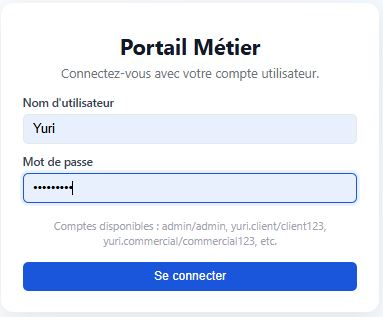
\includegraphics[width=0.75\textwidth]{Chap4/images/image6.JPG}
\caption{Portail de connexion à l'application \texttt{E-commerce\_Application}}
\label{fig:chap4-portail-connexion}
\end{figure}

\begin{figure}[H]
\centering
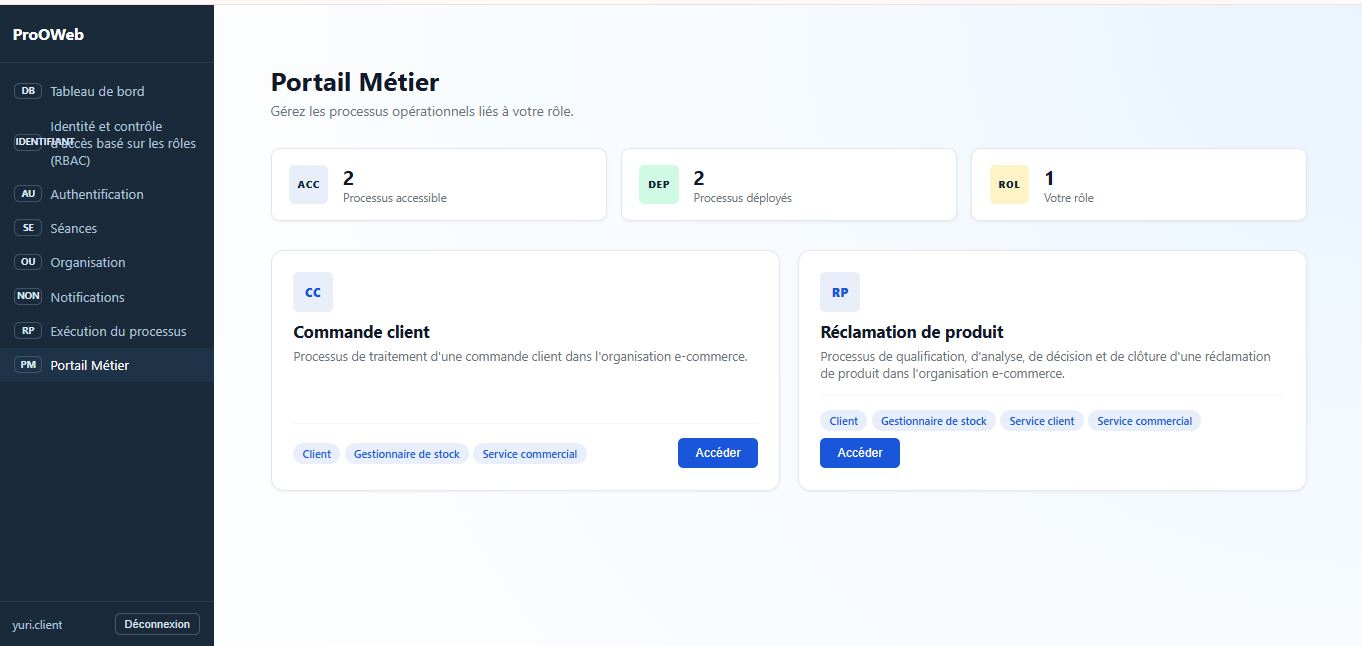
\includegraphics[width=0.75\textwidth]{Chap4/images/image7.JPG}
\caption{Tableau de bord pour un utilisateur connecté avec le rôle \texttt{CLIENT}}
\label{fig:chap4-dashboard-client}
\end{figure}

\begin{figure}[H]
\centering
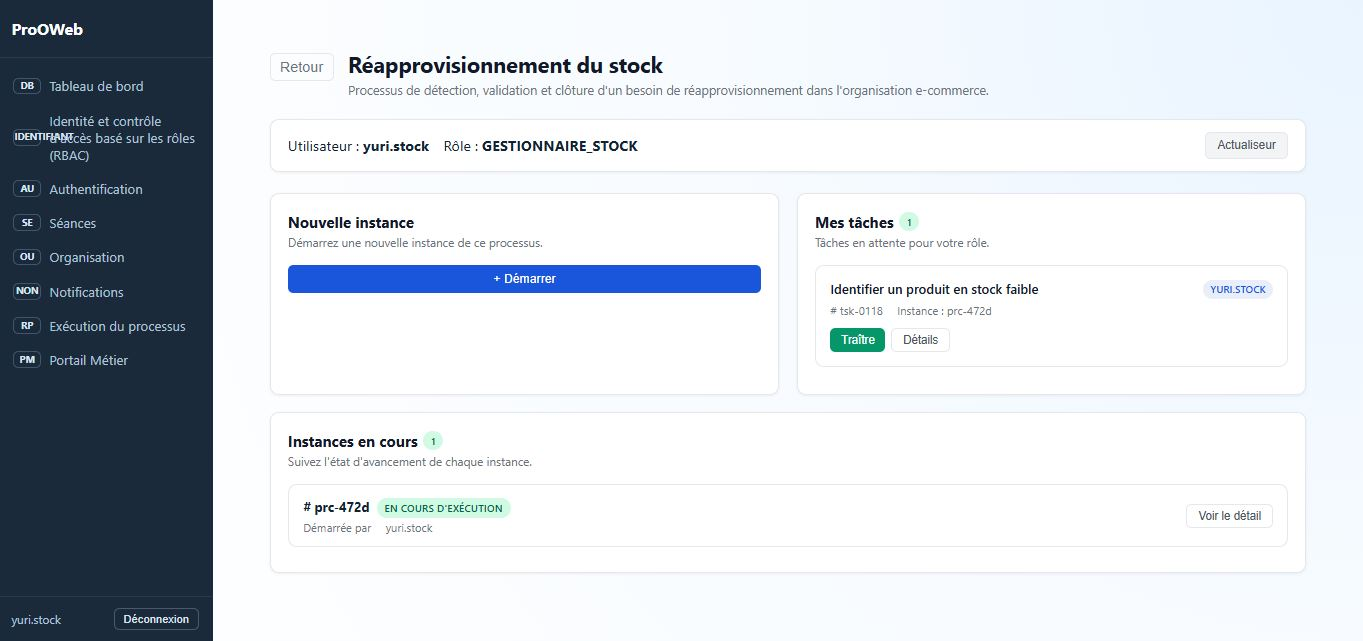
\includegraphics[width=0.75\textwidth]{Chap4/images/image9.JPG}
\caption{Tableau de bord pour un utilisateur connecté avec le rôle \texttt{GESTIONNAIRE\_STOCK}}
\label{fig:chap4-dashboard-stock}
\end{figure}

\begin{figure}[H]
\centering
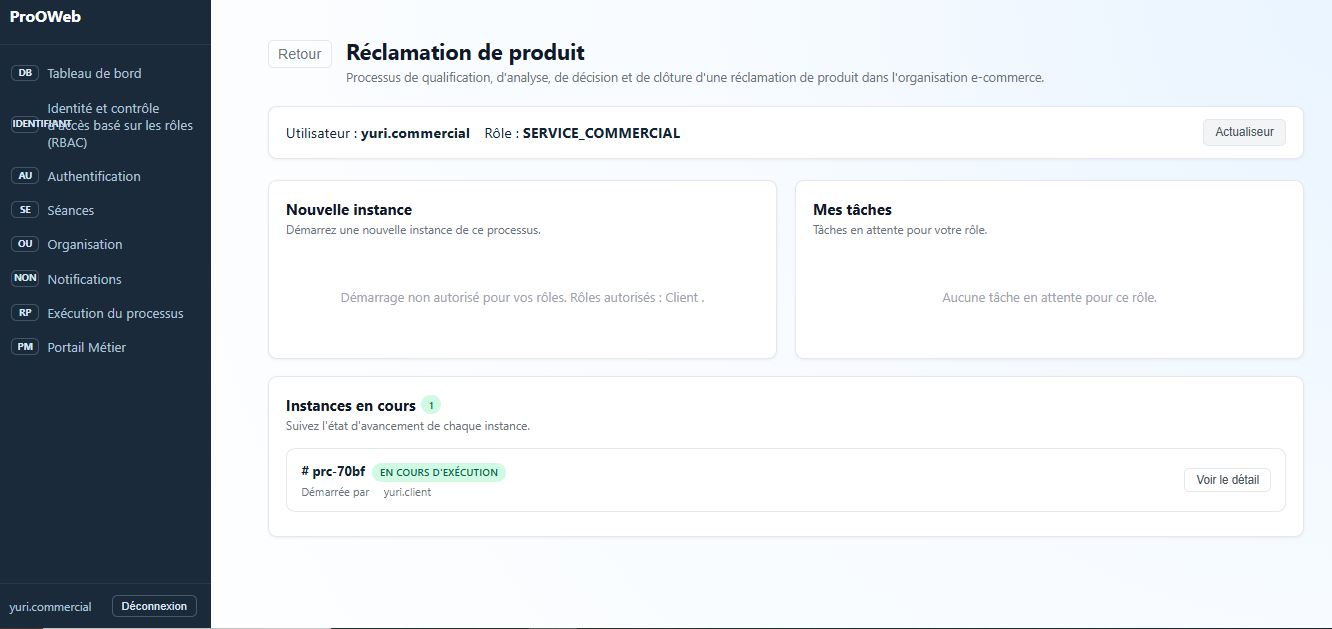
\includegraphics[width=0.75\textwidth]{Chap4/images/image10.JPG}
\caption{Tableau de bord pour un utilisateur connecté avec le rôle \texttt{SERVICE\_COMMERCIAL}}
\label{fig:chap4-dashboard-commercial}
\end{figure}
%Cette unité applicative constitue un résultat important du cas pratique. Les processus restent distincts du point de vue métier, mais ils partagent un socle commun : authentification, rôles, registre de processus, listes de tâches, historique, supervision et données métier communes. C'est précisément ce comportement qui permet de parler d'une application organisationnelle, et non d'un simple générateur de formulaires.

%\begin{table}[H]
%\centering
%\caption{Fonctions observées dans l'application générée}
%\label{tab:chap4-fonctions-observees}
%\begin{tabularx}{\textwidth}{p{4.0cm}X}
%\toprule
%\textbf{Fonction observée} & \textbf{Manifestation dans le cas pratique} \\
%\midrule
%Registre des processus & Les processus de commande, de réapprovisionnement et de réclamation sont accessibles dans le même environnement applicatif. \\
%Listes de tâches & Les tâches visibles dépendent du rôle connecté : service commercial, stock, achats ou service client. \\
%Formulaires d'activité & Les champs affichés correspondent aux données de commande, produit, stock ou réclamation déclarées dans \textit{spec-v1}. \\
%Progression des instances & Les statuts changent selon les transitions issues des modèles BPMN propres à chaque processus. \\
%Supervision & Les commandes, réapprovisionnements, réclamations et décisions restent consultables par les rôles autorisés. \\
%\bottomrule
%\end{tabularx}
%\end{table}

\mySection{Évaluation de ProOWeb}{}
\label{sec:chap4-evaluation}

\subsection{Méthode d'évaluation}

L'évaluation menée dans ce chapitre est fonctionnelle et qualitative. Elle vérifie si ProOWeb permet de générer une application web métier exploitable à partir de plusieurs processus d'une même organisation. Les critères retenus découlent directement des objectifs du chapitre précédent : exploiter BPMN et \textit{spec-v1}, produire des artefacts applicatifs cohérents, préserver la traçabilité et permettre une évolution contrôlée.

La méthode croise l'inspection des artefacts produits et l'observation du comportement de l'application générée. Les fichiers BPMN conservés, les contrats \texttt{runtime}, les contrats \texttt{data}, le catalogue global et les classes générées côté backend permettent de vérifier ce que ProOWeb a réellement produit. Les tests Cypress complètent cette lecture : ils ouvrent le \textit{Process Runtime Workbench}, démarrent une instance de processus, complètent les tâches du parcours nominal et vérifient l'état final de l'instance.

\begin{table}[H]
\centering
\caption{Critères retenus pour l'évaluation}
\label{tab:chap4-criteres-evaluation}
\begin{tabularx}{\textwidth}{p{3.1cm}p{4.8cm}X}
\toprule
\textbf{Critère} & \textbf{Question posée} & \textbf{Mode d'observation} \\
\midrule
Complétude fonctionnelle & Les éléments nécessaires au runtime de processus sont-ils produits ? & Analyse des ressources générées, des contrats et des classes backend. \\
Cohérence BPMN-application & Les activités du modèle apparaissent-elles dans les contrats et les parcours testés ? & Comparaison entre BPMN, contrats \texttt{runtime} et tests Cypress. \\
Gestion des rôles & Les rôles de démarrage, de suivi et d'affectation sont-ils projetés ? & Analyse des contrats et des options de démarrage exposées au runtime. \\
Gestion des données & Les données partagées et les sorties d'activités sont-elles prises en compte ? & Vérification des contrats \texttt{data} et des entités partagées. \\
Capacité multi-processus & L'application regroupe-t-elle plusieurs processus dans un même environnement ? & Observation du catalogue, des ressources déployées et des tests par processus. \\
Évolution contrôlée & Les fichiers générés restent-ils identifiables après déploiement ? & Analyse du manifeste et des ressources suivies. \\
\bottomrule
\end{tabularx}
\end{table}

\subsection{Résultats observés}

Les résultats observés se situent à deux niveaux. Au niveau du framework, ProOWeb lit les modèles, valide les informations, produit les contrats et écrit les artefacts du projet cible. Au niveau de l'application générée, les utilisateurs disposent d'un environnement de runtime dans lequel une instance de processus peut être créée, suivie et terminée selon les tâches exposées.

Le tableau suivant synthétise les observations réalisées sur le cas pratique. Il ne prétend pas mesurer toutes les qualités possibles d'un système d'information ; il montre ce que la mise en oeuvre permet déjà de vérifier par rapport aux objectifs du mémoire.

\begin{table}[H]
\centering
\caption{Synthèse des résultats observés sur le cas d'étude}
\label{tab:chap4-resultats-observes}
\begin{tabularx}{\textwidth}{p{3.1cm}p{4.2cm}X}
\toprule
\textbf{Élément évalué} & \textbf{Résultat observé} & \textbf{Interprétation} \\
\midrule
Ressources de processus & Les trois processus disposent chacun d'un BPMN, d'une spécification, d'un contrat runtime et d'un contrat data. & ProOWeb conserve le lien entre la source métier et les artefacts projetés. \\
Catalogue global & Les catalogues runtime et data regroupent les versions déployées. & L'application générée peut raisonner sur plusieurs processus dans un même socle. \\
Backend généré & Des classes telles que le registre de processus et les spécifications Java sont générées côté Spring Boot. & Les processus ne restent pas confinés à des fichiers de configuration. \\
Runtime frontend & Les tests utilisent le \textit{Process Runtime Workbench} pour démarrer et terminer des instances. & Le frontend généré sait consommer les options de démarrage, les tâches et la progression d'une instance. \\
Tests e2e & Trois tests Cypress sont dédiés aux parcours de commande, de réapprovisionnement et de réclamation. & Chaque processus fait l'objet d'un parcours nominal vérifiable. \\
Manifeste & Les fichiers produits restent identifiés comme éléments gérés par ProOWeb. & La régénération peut être analysée au lieu d'être subie. \\
\bottomrule
\end{tabularx}
\end{table}

\begin{table}[H]
\centering
\caption{Parcours vérifiés par les tests Cypress}
\label{tab:chap4-parcours-cypress}
\begin{tabularx}{\textwidth}{p{3.8cm}p{4.1cm}X}
\toprule
\textbf{Processus testé} & \textbf{Parcours nominal vérifié} & \textbf{État attendu} \\
\midrule
Commande client & Démarrage de l'instance, passage de commande, vérification des informations de commande & Instance terminée avec le marqueur \texttt{INSTANCE\_COMPLETED}. \\
Réapprovisionnement du stock & Identification d'un produit en stock faible, création de la demande, examen de la demande & Instance terminée avec le marqueur \texttt{INSTANCE\_COMPLETED}. \\
Réclamation de produit & Dépôt de la réclamation, qualification, vérification de la commande concernée & Instance terminée avec le marqueur \texttt{INSTANCE\_COMPLETED}. \\
\bottomrule
\end{tabularx}
\end{table}

\subsection{Analyse de la capacité multi-processus}

La capacité multi-processus occupe une place centrale dans cette évaluation, car elle touche directement à l'ambition de ProOWeb. Une application métier n'est pas seulement une suite d'écrans attachés à une procédure. Elle doit porter une partie de la vie de l'organisation, avec ses acteurs, ses données partagées et ses décisions qui se répondent d'un processus à l'autre.

Dans le cas d'étude, les trois processus ne sont donc pas juxtaposés au hasard. La commande client sollicite le stock ; le réapprovisionnement agit sur la disponibilité des produits ; la réclamation de produit se rattache à une commande déjà enregistrée et peut impliquer le service client, le service commercial ou le gestionnaire de stock. Cette proximité donne du sens au test réalisé : chaque processus conserve son propre déroulement, ses activités et ses transitions, tandis que l'application générée garde un socle commun pour les rôles, les tâches, l'historique, les produits et la supervision.

Ce résultat montre que ProOWeb peut soutenir une logique d'application organisationnelle. Les processus restent identifiables, mais ils ne sont pas enfermés dans trois applications séparées. L'utilisateur travaille dans un même environnement et l'application peut exposer les tâches selon les responsabilités déclarées dans les modèles et les spécifications.

\subsection{Apports observés}

L'évaluation met surtout en évidence la continuité obtenue entre la modélisation et l'application produite. Les activités décrites dans les modèles ne restent pas au niveau de la documentation : elles se retrouvent dans les tâches, les vues, les actions de traitement et les transitions du runtime. Cette continuité réduit le risque de voir le logiciel s'éloigner progressivement du processus métier qui l'a justifié.

\textit{spec-v1} joue également un rôle important. Les rôles, les données manipulées, les règles de visibilité et les sorties d'activités ne sont pas ajoutés tardivement dans le code ; ils sont déclarés avant la génération et deviennent des éléments exploitables par ProOWeb. Le projet généré gagne ainsi en lisibilité, car les choix métier restent rattachés à une source identifiable.

Un autre apport tient à la structure du résultat obtenu. Le workspace généré n'est pas une accumulation de fichiers difficiles à relier. Il possède une organisation backend/frontend, des contrats de processus, des ressources de données, des scripts de vérification et un manifeste de fichiers gérés. Cette structuration facilite la reprise par un développeur et prépare les évolutions futures du projet.

\subsection{Limites observées}

ProOWeb présente aussi des limites. La qualité des modèles d'entrée reste déterminante : si le BPMN est ambigu ou si la spécification \textit{spec-v1} est incomplète, la génération ne peut pas produire une application correcte. Le framework peut signaler des incohérences, mais il ne remplace pas l'analyse métier.

Certaines règles très spécifiques doivent également être traitées avec prudence. Dans une organisation de commerce électronique réelle, des décisions peuvent dépendre du transporteur, du prestataire de paiement, des promotions, des garanties commerciales ou des accords fournisseurs. Ces comportements nécessitent parfois une extension manuelle. L'évaluation menée ici garde elle aussi un périmètre limité : les tests Cypress vérifient les parcours du \textit{Process Runtime Workbench} avec un backend simulé. Ils sont utiles pour contrôler l'enchaînement frontend/runtime, mais ils ne remplacent pas une campagne complète d'intégration, de charge, de sécurité et de persistance sur une infrastructure réelle.

Enfin, l'application générée reste un socle. Elle réduit la distance entre le modèle métier et le projet applicatif, mais elle ne supprime pas le rôle du développeur. Dans un projet réel, une équipe devra encore enrichir les tests, ajuster l'expérience utilisateur, raccorder les services externes et vérifier les règles métier propres à son environnement.

\subsection{Discussion}

Les résultats obtenus permettent de situer ProOWeb comme un framework de génération d'applications web métier pilotées par BPMN. Ils confirment, sur le cas e-commerce étudié, la logique défendue au chapitre précédent : BPMN décrit le déroulement métier, \textit{spec-v1} complète les informations applicatives, les contrats intermédiaires stabilisent la génération et le manifeste prépare l'évolution. Sa valeur ne réside pas seulement dans la production de fichiers, mais dans la cohérence qu'il maintient entre processus, rôles, données, interfaces et suivi de génération.

Le cas pratique montre également que la spécification enrichie joue un rôle déterminant. BPMN décrit le déroulement du travail, mais l'application a besoin d'informations supplémentaires. En rendant ces informations explicites dans \textit{spec-v1}, ProOWeb rend la génération plus contrôlable. Cet effort de spécification est le prix à payer pour produire une application métier plus complète qu'une simple maquette d'interface.

\mySection{Conclusion}{}

Ce chapitre a présenté la mise en oeuvre de ProOWeb et son application à un cas d'étude centré sur une organisation de commerce électronique. Il a montré comment les modèles BPMN enrichis sont importés, validés, transformés en contrats, puis déployés dans une application web métier générée.

Le cas pratique a permis d'observer ProOWeb sur trois processus appartenant au même contexte : commande client, réapprovisionnement du stock et réclamation de produit. L'évaluation confirme l'intérêt du framework pour produire une base applicative cohérente et multi-processus, tout en rappelant ses limites : qualité nécessaire des modèles d'entrée, effort de spécification, tests encore centrés sur des parcours nominaux et besoin d'évaluations complémentaires sur des environnements plus proches de la production.
